\documentclass[12pt]{beamer}
\usepackage{../Estilos/BeamerMAF}
\usepackage{../Estilos/ColoresLatex}
\usetheme{Warsaw}
\usecolortheme{seahorse}
%\useoutertheme{default}
\setbeamercovered{invisible}
% or whatever (possibly just delete it)
\setbeamertemplate{section in toc}[sections numbered]
\setbeamertemplate{subsection in toc}[subsections numbered]
\setbeamertemplate{subsection in toc}{\leavevmode\leftskip=3.2em\rlap{\hskip-2em\inserttocsectionnumber.\inserttocsubsectionnumber}\inserttocsubsection\par}
\setbeamercolor{section in toc}{fg=blue}
\setbeamercolor{subsection in toc}{fg=blue}
\setbeamercolor{frametitle}{fg=blue}
\setbeamertemplate{caption}[numbered]

\setbeamertemplate{footline}
\beamertemplatenavigationsymbolsempty
\setbeamertemplate{headline}{}


\makeatletter
\setbeamercolor{section in foot}{bg=gray!30, fg=black!90!orange}
\setbeamercolor{subsection in foot}{bg=blue!30}
\setbeamercolor{date in foot}{bg=black}
\setbeamertemplate{footline}
{
  \leavevmode%
  \hbox{%
  \begin{beamercolorbox}[wd=.333333\paperwidth,ht=2.25ex,dp=1ex,center]{section in foot}%
    \usebeamerfont{section in foot} \insertsection
  \end{beamercolorbox}%
  \begin{beamercolorbox}[wd=.333333\paperwidth,ht=2.25ex,dp=1ex,center]{subsection in foot}%
    \usebeamerfont{subsection in foot}  \insertsubsection
  \end{beamercolorbox}%
  \begin{beamercolorbox}[wd=.333333\paperwidth,ht=2.25ex,dp=1ex,right]{date in head/foot}%
    \usebeamerfont{date in head/foot} \insertshortdate{} \hspace*{2em}
    \insertframenumber{} / \inserttotalframenumber \hspace*{2ex} 
  \end{beamercolorbox}}%
  \vskip0pt%
}
\makeatother

\makeatletter
\patchcmd{\beamer@sectionintoc}{\vskip1.5em}{\vskip0.8em}{}{}
\makeatother

\newlength{\depthofsumsign}
\setlength{\depthofsumsign}{\depthof{$\sum$}}
\newcommand{\nsum}[1][1.4]{% only for \displaystyle
    \mathop{%
        \raisebox
            {-#1\depthofsumsign+1\depthofsumsign}
            {\scalebox
                {#1}
                {$\displaystyle\sum$}%
            }
    }
}
\def\scaleint#1{\vcenter{\hbox{\scaleto[3ex]{\displaystyle\int}{#1}}}}
\def\scaleoint#1{\vcenter{\hbox{\scaleto[3ex]{\displaystyle\oint}{#1}}}}
\def\bs{\mkern-12mu}

\usepackage{pifont}

\AtBeginDocument{\RenewCommandCopy\qty\SI}
\ExplSyntaxOn
\msg_redirect_name:nnn { siunitx } { physics-pkg } { none }
\ExplSyntaxOff


\title{\large{1 - Coordenadas curvilíneas ortogonales}}
\subtitle{Tema 1 - La física y la geometría}

\author{M. en C. Gustavo Contreras Mayén}
\date{}

\begin{document}
\maketitle
\fontsize{14}{14}\selectfont

\section*{Contenido}
\frame{\frametitle{Contenido} \tableofcontents[currentsection, hideallsubsections]}

\section{Coordenadas curvilíneas ortogonales}
\frame{\tableofcontents[currentsection, hideothersubsections]}
\subsection{Introducción}

%Ref. Sepúlveda (2004) - 1 Coord. curvilíneas ortogonales
\begin{frame}
\frametitle{Coordenadas cartesianas}
En el espacio euclidiano tridimensional las coordenadas cartesianas se definen en términos de tres familias de planos perpendiculares: 
\begin{align*}
x = x_{0}, \hspace{0.25cm} y = y_{0}, \hspace{0.25cm} z = z_{0}
\end{align*}
\pause
Como vemos en la figura \ref{fig:figura_planos_cartesianos}:
\end{frame}
\begin{frame}
\frametitle{Coordenadas cartesianas}
\begin{figure}[h!]
   \centering
   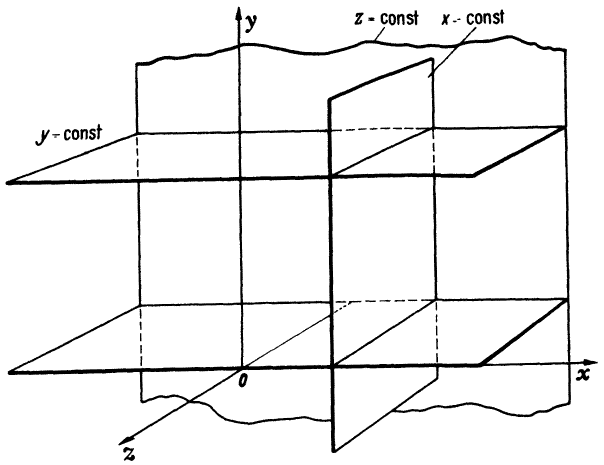
\includegraphics[scale=1.3]{Imagenes/Planos_Coordenadas_Cartesianas.png}
   \caption{Las superficies coordenadas son los planos $x=\mbox{cte.}, y=\mbox{cte.}, z=\mbox{cte.}$}
   \label{fig:figura_planos_cartesianos}
\end{figure}
\end{frame}
\begin{frame}
\frametitle{Coordenadas cartesianas}
La intersección de los planos $x = x_{0}$ y $y = y_{0}$ genera una línea recta paralela al eje $z$
que pasa por el punto $(x_{0}, y_{0}, 0)$.
\end{frame}
\begin{frame}
\frametitle{Coordenadas cartesianas}
La intersección de los tres planos $x = x_{0}, y = y_{0}, z = z_{0}$ genera un punto de coordenadas $(x_{0}, y_{0}, z_{0})$.
\end{frame}
\begin{frame}
\frametitle{Coordenadas esféricas}
Las coordenadas esféricas se definen en términos de tres superficies: esferas concéntricas, conos con el mismo vértice y planos meridianos.
\\
\bigskip
\pause
Un punto tiene coordenadas $(r, \theta, \phi)$ y las tres superficies son perpendiculares en cada punto.
\end{frame}
\begin{frame}
\frametitle{Coordenadas esféricas}
\begin{figure}[h!]
   \centering
   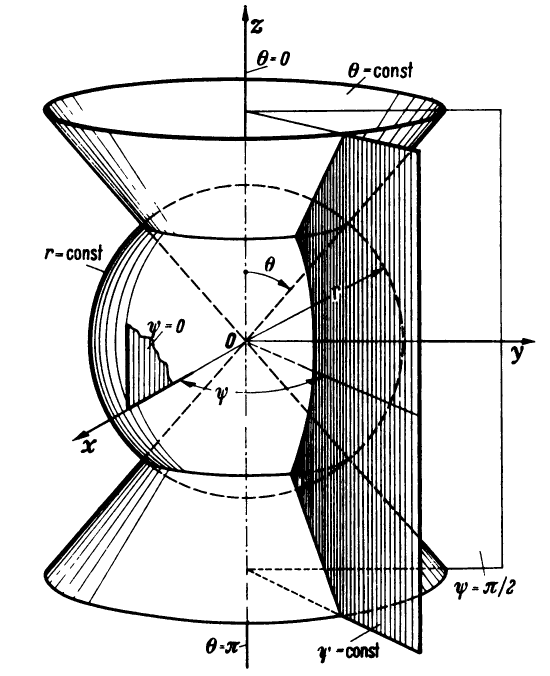
\includegraphics{Imagenes/Planos_Coordenadas_Esfericas.png}
   \caption{Coordenadas esféricas $(r, \theta, \phi)$. Las superficies coordenadas son \emph{esferas} ($r = \mbox{cte.}$), \emph{conos circulares} $(\theta = \mbox{const})$, \emph{planos meridianos} $(\phi = \mbox{cte.})$}
   \label{fig:figura_planos_esfericos}
\end{figure}
\end{frame}
\begin{frame}
\frametitle{Coordenadas esféricas}
La intersección del cono y la esfera genera una circunferencia a lo largo de la cual varía
sólo la coordenada $\phi$.
\\
\bigskip
\pause
La intersección de la esfera y el plano meridiano genera un arco de meridiano a lo largo del cual sólo $\theta$ varía, y la intersección del cono y el plano genera una recta radial a lo largo de la cual sólo $r$ varía.
\end{frame}
\begin{frame}
\frametitle{Coordenadas esféricas}
La conexión entre coordenadas cartesianas y esféricas (regla de transformación) tiene la forma:
\begin{align*}
x &= r \, \sin \theta \cos \varphi \\
y &= r \sin \theta \sin \varphi \\
z &= r \cos \theta
\end{align*}
\end{frame}
\begin{frame}
\frametitle{Otros sistemas coordenados}
De manera análoga tenemos que para las coordenadas cilíndricas, se construyen con tres superficies perpendiculares: cilindros concéntricos, planos meridianos y planos horizontales, como se ve en la figura \ref{fig:figura_planos_cilindricos}.
\\
\bigskip
\pause
A cada una se le asocian, las coordenadas $(\rho, \phi, z)$ respectivamente.
\end{frame}
\begin{frame}
\frametitle{Sistema cilíndrico}
\begin{figure}[h!]
   \centering
   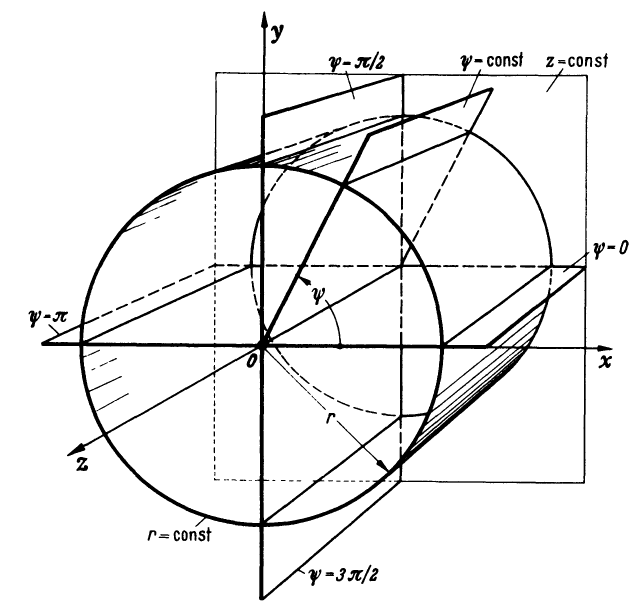
\includegraphics{Imagenes/Planos_Coordenadas_Cilindricas.png}
   \caption{Coordenadas cilíndricas $(\rho, \theta, z)$. Las superficies coordenadas son \emph{cilindros circulares} ($\rho = \mbox{cte.}$), \emph{planos meridianos} $(\theta = \mbox{const})$ que intersectan al eje $x$, \emph{planos paralelos} $(z = \mbox{cte.})$}
   \label{fig:figura_planos_cilindricos}
\end{figure}
\end{frame}
\begin{frame}
\frametitle{Sistema cilíndrico}
Las reglas de transformación entre coordenadas cartesianas y cilíndricas son de la forma:
\begin{align*}
x &= \rho \, \cos \phi \\ 
y &= \rho \, \sin \phi \\
z &= z
\end{align*}
\end{frame}

\subsection{Coordenadas curvilíneas ortogonales}

\begin{frame}
\frametitle{Generalización}
Una generalización directa permite pensar en tres familias de superficies, en general curvas, que en cada punto del espacio se intersectan en ángulo recto.
\end{frame}
\begin{frame}
\frametitle{Generalización}
Estas superficies pueden describirse mediante las ecuaciones:
\begin{align*}
u_{1} &= f_{1}(x, y, z) \\
u_{2} &= f_{2}(x, y, z) \\
u_{3} &= f_{3}(x, y, z)
\end{align*}
\end{frame}
\begin{frame}
\frametitle{Generalización}
Equivalentemente:
\begin{align*}
x &= x(u_{i}) \\
y &= y(u_{i}) \\
z &= z(u_{i})
\end{align*}
\pause
Estas ecuaciones son a la vez las reglas de transformación entre \textocolor{ao}{coordenadas cartesianas} y las \textocolor{byzantine}{coordenadas curvilíneas ortogonales}.
\end{frame}
\begin{frame}
\frametitle{Generalización}
Las superficies $u_{1} = \mbox{cte.}$ y $u_{2} = \mbox{cte.}$ se intersectan en una curva a lo largo de la cual solo $u_{3}$ varía, esta curva define a la coordenada $u_{3}$, como se ve en la figura \ref{fig:figura_Sistema_Curvilineo_Ortogonal}.
\end{frame}
\begin{frame}
\begin{figure}[h!]
   \centering
   \includestandalone[scale=0.8]{Figuras/Sistema_Curvilineo_Ortogonal}
   \caption{Sistema curvilíneo ortogonal. Los vectores unitarios $(\vu{e}_{1}, \vu{e}_{2}, \vu{e}_{3})$ son tangentes a las superficies.}
   \label{fig:figura_Sistema_Curvilineo_Ortogonal}
\end{figure}
\end{frame}
\begin{frame}
   \frametitle{Generalización}
Análogamente las superficies $u_{1} = \mbox{cte.}$ y $u_{3} = \mbox{cte.}$ generan la curva $u_{2}$; y las superficies $u_{2} = \mbox{cte.}$ y $u_{3} = \mbox{cte.}$ generan la curva $u_{1}$.
\end{frame}
\begin{frame}
\frametitle{Generalización}   
La intersección de las tres superficies genera un punto cuyas coordenadas son $(u_{1}, u_{2}, u_{3})$.
\\
\bigskip
\pause
Dado un punto $(x, y, z)$ es posible asignarle unívocamente un conjunto $(u_{1}, u_{2}, u_{3})$ de coordenadas curvilíneas.
\end{frame}
\begin{frame}
\frametitle{Características del sistema coordenado}
El sistema de coordenadas curvilíneas construido con estas superficies, tiene las siguientes características:
\pause
\setbeamercolor{item projected}{bg=lava,fg=white}
\setbeamertemplate{enumerate items}{%
\usebeamercolor[bg]{item projected}%
\raisebox{1.5pt}{\colorbox{bg}{\color{fg}\footnotesize\insertenumlabel}}%
}
\begin{enumerate}[<+->]
\item Los ejes coordenados son en general curvas que se intersectan en ángulo recto, de modo que los vectores unitarios $\left\{ \vu{e}_{i} \right\}$, que son tangentes a las curvas, generan una base ortonormal tridimensional.
\seti
\end{enumerate}
\end{frame}
\begin{frame}
\frametitle{Característica del sistema coordenado}
En el curso nos enfocaremos en el estudio de este tipo de sistemas: coordenados ortogonales, los sistemas coordenados no ortogonales no los revisaremos.
\end{frame}
\begin{frame}
\frametitle{Características del sistema coordenado}
\setbeamercolor{item projected}{bg=lava,fg=white}
\setbeamertemplate{enumerate items}{%
\usebeamercolor[bg]{item projected}%
\raisebox{1.5pt}{\colorbox{bg}{\color{fg}\footnotesize\insertenumlabel}}%
}
\begin{enumerate}[<+->]
\conti
\item La orientación de la base $\left\{ \vu{e}_{i} \right\}$ puede cambiar de punto a punto, preservándose su ortonormalidad.
\item El significado físico de los diferenciales de las coordenadas \emph{no es necesariamente una longitud}. En coordenadas esféricas, tenemos una longitud y dos ángulos.
\end{enumerate}
\end{frame}

\subsection*{Campo escalar}

\begin{frame}
\frametitle{Campo escalar}
Un \textocolor{blue-violet}{campo escalar} se define dando un valor numérico en cada punto del espacio.
\\
\bigskip
\pause
El valor de una cantidad escalar en un punto definido del espacio es independiente
del sistema de coordenadas que se utilice.
\end{frame}
\begin{frame}
\frametitle{Campo escalar}
Por lo que decimos que si $(x, y, z)$, $(\rho, \phi, z)$, $(r, \theta, \phi)$ denotan el mismo punto del espacio físico, el valor que en ese punto tome, por ejemplo, la presión atmosférica es el mismo.
\end{frame}

\subsection*{Campo vectorial}

\begin{frame}
\frametitle{Campo vectorial}
Los \textocolor{brown(web)}{campos vectoriales} se definen dando en cada punto del espacio el valor de tres cantidades, conocidas como las \emph{componentes vectoriales}.
\end{frame}
\begin{frame}
\frametitle{Campo vectorial}
Aunque los vectores unitarios y los valores de cada componente sean diferentes en cada sistema de coordenadas, es sin embargo cierto que el vector $\vb{A}$ no cambia cuando cambiamos de sistema coordenado.
\end{frame}
\begin{frame}
\frametitle{Campo vectorial}
Por lo que podemos decir que si los vectores unitarios $\vu{e}_{i}$ y $\vu{e}_{i}^{\prime}$, y las componentes $A_{i}$ y $A_{i}^{\prime}$ en dos sistemas coordenados $S$ y $S^{\prime}$, entonces:
\pause
\begin{align*}
\vb{A} = \nsum_{i=1}^{3} A_{i} \, \vu{e}_{i} = \nsum_{i=1}^{3} A_{i}^{\prime} \, \vu{e}_{i}^{\prime}
\end{align*}
\end{frame}
\begin{frame}
\frametitle{Vectores invariantes}
Esto significa que un vector es \textocolor{burgundy}{invariante} bajo transformaciones de coordenadas.
\\
\bigskip
\pause
Los campos escalares son también invariantes bajo transformaciones de coordenadas. En la \emph{teoría de transformación} se revisa estos temas.
\end{frame}

\subsection*{Ecuaciones matemáticas}

\begin{frame}
\frametitle{Ecuaciones matemáticas}
De esta manera es posible escribir ecuaciones cuya forma matemática es la misma en todos los sistemas de coordenadas en el espacio 3D euclidiano.
\end{frame}
\begin{frame}
\frametitle{Ecuaciones matemáticas}
Por ejemplo, la ecuación de onda:
\begin{align*}
\laplacian{\psi} - \dfrac{1}{v^{2}} \pdv[2]{\psi}{t} = 0
\end{align*}
es válida en todos los sistemas coordenados, es decir, es invariante bajo transformación de coordenadas.
\end{frame}

\section{Teoría de transformación}
\frame{\tableofcontents[currentsection, hideothersubsections]}
\subsection{Construcción}

\begin{frame}
\frametitle{Construcción}
En el espacio euclidiano es siempre posible construir un sistema coordenado cartesiano que se extienda indefinidamente.
\\
\bigskip
\pause
A partir de él podemos generar múltiples sistemas coordenados, mediante el uso de las superficies $u_{i} = f(x, y, z)$
\end{frame}
\begin{frame}
\frametitle{Construcción}
Dado que de manera recíproca, $(x, y, z)$ son funciones de $u_{i}$, es decir:
\begin{align*}
x &= x(u_{i}) \\
y &= y(u_{i}) \\
z &= z(u_{i})
\end{align*}
\end{frame}
\begin{frame}
\frametitle{Construcción}
Entonces podemos escribir:
\pause
% se usa eqnarray para que funcione la pausa
\begin{eqnarray*}
\dd{x} = \pdv{x}{u_{1}} \dd{u_{1}} + \pdv{x}{u_{2}} \dd{u_{2}} + \pdv{x}{u_{3}} \dd{u_{3}} \\[0.5em]
\pause
\dd{y} = \pdv{y}{u_{1}} \dd{u_{1}} + \pdv{y}{u_{2}} \dd{u_{2}} + \pdv{y}{u_{3}} \dd{u_{3}} \\[0.5em]
\pause
\dd{z} = \pdv{z}{u_{1}} \dd{u_{1}} + \pdv{z}{u_{2}} \dd{u_{2}} + \pdv{z}{u_{3}} \dd{u_{3}} \\
\end{eqnarray*}
\end{frame}
\begin{frame}
\frametitle{Ecuación vectorial}
Estas tres ecuaciones son las componentes de la ecuación vectorial:
\pause
\begin{align}
\begin{aligned}
\dd{\vb{r}} &= \pdv{\vb{r}}{u_{1}} \dd{u_{1}} + \pdv{\vb{r}}{u_{2}} \dd{u_{2}} + \pdv{\vb{r}}{u_{3}} \dd{u_{3}} = \\[0.5em]
&= \nsum_{i=1}^{3} \pdv{\vb{r}}{u_{i}} \dd{u_{i}}
\end{aligned}
\label{eq:ecuacion_01_01}
\end{align}
\end{frame}
\begin{frame}
\frametitle{Vector no unitario}
En general, el factor $\pdv*{\vb{r}}{u_{i}}$ en la ec. (\ref{eq:ecuacion_01_01}) es un vector \emph{no unitario} que toma en cuenta la variación de $\vb{r}$ solo en la dirección de $u_{i}$, y es por tanto, tangente a la curva coordenada $u_{i}$.
\end{frame}
\begin{frame}
\frametitle{Base normalizada}
Con el fin de introducir una \emph{base normalizada} $\vu{e}_{i}$, es decir, un conjunto de vectores unitarios, escribimos:
\pause
\begin{align}
\pdv{\vb{r}}{u_{i}} = h_{i} \, \vu{e}_{i}
\label{eq:ecuacion_01_02}
\end{align}
\pause
donde $\abs{\vb{e}_{i}} = 1$ y $h_{i}$ son funciones de $u_{i}$, que llamaremos \textocolor{cobalt}{factores de escala}.
\end{frame}
\begin{frame}
\frametitle{Diferencial de desplazamiento}
Se sigue entonces que el diferencial de desplazamiento es:
\pause
\begin{align*}
\dd{\vb{r}} = \nsum_{i=1}^{3} h_{i} \, \vu{e}_{i} \dd{u_{i}}
\end{align*}
\end{frame}
\begin{frame}
\frametitle{Bases ortonormales}
Como hicimos la aclaración de trabajar con bases \emph{ortonormales} (perpendiculares y unitarias), podemos escribir:
\pause
\begin{align}
\vu{e}_{i} \cdot \vu{e}_{j} = \delta_{ij}
\label{eq:ecuacion_01_03}
\end{align}
donde $\delta_{ij}$ es la delta de Kronecker:
\pause
\begin{align*}
\delta_{ij} = 
\begin{cases}
0 & \mbox{si } i \neq j \\
1 & \mbox{si } i = j
\end{cases}
\end{align*}
\end{frame}
\begin{frame}
\frametitle{Bases ortonormales}
Entonces tendremos que:
\pause
\begin{align*}
\vu{e}_{1} \cdot \vu{e}_{2} = \vu{e}_{2} \cdot \vu{e}_{3} = \vu{e}_{3} \cdot \vu{e}_{1} = 0  
\end{align*}
y además:
\pause
\begin{align*}
\vu{e}_{1} \cdot \vu{e}_{1} = \abs{\vu{e}_{1}}^{2} = \abs{\vu{e}_{2}}^{2} = \abs{\vu{e}_{3}}^{2} = 1
\end{align*}
\end{frame}
\begin{frame}
\frametitle{Definición del factor de escala}
Por la ecuación (\ref{eq:ecuacion_01_02}), los factores de escala se definen por:
\pause
\begin{align}
\abs{\pdv{\vb{r}}{u_{i}}} = h_{i}
\label{eq:ecuacion_01_04}
\end{align}
por lo que es fácil calcular los factores de escala.
\end{frame}
\begin{frame}
\frametitle{Vectores unitarios}
En consecuencia los vectores unitarios en coordenadas curvilíneas (ec. \ref{eq:ecuacion_01_02}) se escriben como:
\pause
\begin{align}
\vu{e}_{i} = \dfrac{1}{h_{i}} \, \pdv{\vb{r}}{u_{i}}
\label{eq:ecuacion_01_05}
\end{align}
\end{frame}

\subsection*{Cambio de coordenadas}

\begin{frame}
\frametitle{Cambio a coordenadas esféricas}
Como ejemplo haremos el cambio de coordenadas cartesianas a coordenadas esféricas.
\begin{align*}
(x, y, z) \longrightarrow (r, \theta, \varphi)
\end{align*}
\end{frame}
\begin{frame}
\frametitle{Cambio a coordenadas esféricas}
Un punto $P$ puede localizarse mediante las coordenadas cartesianas $(x, y, z)$ y también mediante coordenadas esféricas $(r, \theta, \varphi)$, donde:
\pause
\begin{minipage}{0.4\linewidth}
\begin{align*}
-\infty \le x \le \infty \\
-\infty \le y \le \infty \\
-\infty \le z \le \infty
\end{align*}
\end{minipage}
\hspace{0.3cm}
\begin{minipage}{0.4\linewidth}
\begin{align*}
r \geq 0 \\
0 \le \theta \le \pi \\
0 \le \varphi \le 2 \, \pi
\end{align*}
\end{minipage}
\end{frame}
\begin{frame}
\frametitle{Identificación de coordenadas}
Donde:
\pause
\begin{itemize}
\item[\ding{212}] $r = \abs{\vb{r}}$ es la coordenada radial.
\item[\ding{212}] $\theta$ es la coordenada polar.
\item[\ding{212}] $\varphi$ es la coordenada azimutal.
\end{itemize}
\end{frame}
\begin{frame}
\frametitle{Reglas de transformación}
De la figura (\ref{fig:figura_planos_esfericos}) la \enquote{conexión} (regla de transformación)  entre las coordenadas cartesianas y esféricas es:
\end{frame}
\begin{frame}
\frametitle{Reglas de transformación}
\begin{align*}
x &= r \, \sin \theta \, \cos \varphi \\
y &= r \, \sin \theta \, \sin \varphi \\
z &= r \, \cos \theta
\end{align*}
\begin{align*}
r &= \sqrt{x^{2} + y^{2} + z^{2}} \\
\theta &= \cos^{-1} \left( z / \sqrt{x^{2} + y^{2} + z^{2}} \right) \\
\varphi &= \tan^{-1} (y/x)
\end{align*}
\end{frame}
\begin{frame}
\frametitle{Cambio a coordenadas esféricas}
Entonces el vector de posición es:
\pause
\begin{align}
\begin{aligned}
\vb{r} &= \vu{i} \, x + \vu{j} \, y + \vu{k} \, z \\
&= \vu{i} \, r \, \sin \theta \, \cos \varphi + \vu{j} \, r \, \sin \theta \, \sin \varphi + \vu{k} \, r \cos \theta 
\end{aligned}
\label{eq:ecuacion_01_06}
\end{align}
\pause
Por lo que podemos calcular los $\pdv*{\vb{r}}{u_{i}}$.
\end{frame}
\begin{frame}
\frametitle{Calculando el factor $\pdv*{\vb{r}}{r}$}
Entonces tenemos que:
\pause
\begin{align*}
\pdv{\vb{r}}{r} = \vu{i} \, \sin \theta \, \cos \varphi + \vu{j} \, \sin \theta \, \sin \varphi + \vu{k} \, \cos \theta
\end{align*}
Así al calcular la norma:
\pause
\begin{eqnarray*}
\abs{\pdv{\vb{u}}{r}} &=& \sqrt{\sin^{2} \theta \, \cos^{2} \varphi + \sin^{2} \theta \, \sin^{2} \varphi + \cos^{2} \theta} = \\[0.5em] \pause
&=& \sqrt{\sin^{2} \theta \left( \cos^{2} \varphi + \sin^{2} \varphi \right) + \cos^{2} \theta} = \\[0.5em] \pause
&=& \sqrt{\sin^{2} \theta + \cos^{2} \theta} = \\[0.5em] \pause
&=& 1
\end{eqnarray*}
\end{frame}
\begin{frame}
\frametitle{Primer factor de escala}
Entonces por la ec. (\ref{eq:ecuacion_01_04}):
\pause
\begin{align*}
\abs{\pdv{\vb{r}}{u_{i}}} = h_{i}
\end{align*}
Tendremos el primer factor de escala:
\pause
\begin{align*}
h_{1} = h_{r} = 1
\end{align*}
\end{frame}
\begin{frame}
\frametitle{Siguiente factor $\pdv*{\vb{r}}{\theta}$}
\begin{align*}
\pdv{\vb{r}}{\theta} = \vu{i} \, r \, \cos \theta \, \cos \varphi + \vu{j} \, r \, \cos \theta \, \sin \varphi - \vu{k} \, r \, \sin \theta
\end{align*}
\pause
Entonces:
\begin{align*}
\abs{\pdv{\vb{u}}{\theta}} &= \sqrt{r^{2} (\cos^{2} \theta \, \cos^{2} \varphi + \cos^{2} \theta \, \sin^{2} \varphi + \sin^{2} \theta)} \\[0.5em]
&= r
\end{align*}
\pause
Así: $h_{2} = h_{\theta} = r$
\end{frame}
\begin{frame}
\frametitle{Siguiente factor $\pdv*{\vb{r}}{\varphi}$}
\begin{align*}
\pdv{\vb{r}}{\varphi} = - \vu{i} \, r \, \sin \theta \, \sin \varphi + \vu{j} \, r \, \sin \theta \, \cos \varphi
\end{align*}
\pause
Entonces:
\begin{align*}
\abs{\pdv{\vb{u}}{\varphi}} &= \sqrt{r^{2} (\sin^{2} \theta \, \sin^{2} \varphi + \sin^{2} \theta \, \cos^{2} \varphi)} \\[0.5em]
&= r \, \sin \theta
\end{align*}
\pause
Así: $h_{3} = h_{\varphi} = r \, \sin \theta$
\end{frame}
\begin{frame}
\frametitle{Factores de escala}
Entonces los factores de escala para el sistema coordenado esférico son:
\pause
\begin{align}
\begin{aligned}
h_{r} &= 1 \\[0.5em]
h_{\theta} &= r \\[0.5em]
h_{\varphi} &= r \, \sin \theta
\end{aligned}
\label{eq:ecuacion_01_07}
\end{align}
\end{frame}
\begin{frame}
\frametitle{Vectores unitarios}
Al reemplazar los factores de escala en la ec. (\ref{eq:ecuacion_01_05}), los vectores unitarios en coordenadas esféricas pueden expresarse en términos de coordenadas cartesianas, como:
\pause
\begin{align}
\begin{aligned}
\vu{e}_{r} &= \vu{i} \, \sin \theta \, \cos \varphi + \vu{j} \, \sin \theta \, \sin \varphi + \vu{k} \, \cos \theta \\[0.25em]
\vu{e}_{\theta} &= \vu{i} \, \cos \theta \, \cos \varphi + \vu{j} \, \cos \theta \, \sin \varphi - \vu{k} \, \sin \theta \\[0.25em]
\vu{e}_{\varphi} &= - \vu{i} \, \sin \varphi + \vu{j} \, \cos \varphi
\end{aligned}
\label{eq:ecuacion_01_08}
\end{align}
Donde $(\vu{e}_{1}, \vu{e}_{2}, \vu{e}_{3}) = (\vu{e}_{r}, \vu{e}_{\theta}, \vu{e}_{\varphi})$
\end{frame}
\begin{frame}
\frametitle{Ecuaciones inversas}
Las ecs. (\ref{eq:ecuacion_01_08}) pueden invertirse algebraicamente para expresar los vectores unitarios $\vu{i}, \vu{j}, \vu{k}$ en términos de $\vu{e}_{r}, \vu{e}_{\theta}, \vu{e}_{\varphi}$, tal que:
\end{frame}
\begin{frame}
\frametitle{Ecuaciones inversas}
Las ecuaciones son:
\pause
\begin{align*}
\vu{i} &= \vu{e}_{r} \, \sin \theta \, \cos \varphi + \vu{e}_{\theta} \, \cos \theta \, \cos \varphi - \vu{e}_{\varphi} \, \sin \varphi \\[0.5em]
\vu{j} &= \vu{e}_{r} \, \sin \theta \, \sin \varphi + \vu{e}_{\theta} \, \cos \theta \, \sin \varphi + \vu{e}_{\varphi} \, \cos \varphi \\[0.5em]
\vu{k} &= \vu{e}_{r} \, \cos \theta - \vu{e}_{\theta} \, \sin \theta
\end{align*}
\end{frame}
\begin{frame}
\frametitle{Representación con matrices}
En forma matricial, tenemos que:
\pause
\begin{align*}
\vu{e} = \vb{A} \, \vu{\epsilon} \hspace{1.5cm} \vu{\epsilon} = \tilde{\vb{A}} \, \vu{e}
\end{align*}
donde:
\end{frame}
\begin{frame}
\frametitle{Representación con matrices}
\begin{align*}
\vu{e} = \mqty(
\vu{e}_{1} \\
\vu{e}_{2} \\
\vu{e}_{3})
= \mqty(
\vu{e}_{r} \\
\vu{e}_{\theta} \\
\vu{e}_{\phi}), \hspace{1.5cm}
\vu{\epsilon} = \mqty(
\vu{\epsilon}_{1} \\
\vu{\epsilon}_{2} \\
\vu{\epsilon}_{3}) = \mqty(
\vu{i} \\
\vu{j} \\
\vu{k})
\end{align*}
\end{frame}
\begin{frame}
\frametitle{Representación con matrices}
Mientras que la matriz $\vb{A}$ es:
\pause
\begin{align*}
\vb{A} = \mqty(
\sin \theta \, \cos \phi & \sin \theta \, \sin \phi & \cos \theta \\
\cos \theta \, \cos \phi & \cos \theta \, \sin \phi & - \sin \theta \\
- \sin \phi & \cos \phi & 0
)
\end{align*}
\end{frame}
\begin{frame}
\frametitle{Sobre la matriz $\vb{A}$}
Es cierto que $\vb{A} \, \tilde{\vb{A}} = \vb{I}$, \pause por lo que:
\pause
\begin{itemize}
\item[\ding{212}] La matriz $\vb{A}$ es ortogonal.
\item[\ding{212}] Además $\abs{\vb{A}} = 1$  
\end{itemize}
\end{frame}

% \begin{frame}
% \frametitle{Ejercicio a cuenta}
% Considera la transformación de coordenadas:
% \begin{align*}
% x &= 2 \, u \, v \\[0.5em]
% y &= u^{2} + v^{2} \\[0.5em]
% z &= w
% \end{align*}
% Demuestra que el nuevo sistema de coordenadas \emph{no} es ortogonal.
% \end{frame}

\subsection{Derivadas de vectores unitarios}

\begin{frame}
\frametitle{Derivadas parciales vectores unitarios}
En aplicaciones de análisis vectorial se requiere utilizar las derivadas parciales $\pdv*{\vu{e}_{i}}{u_{j}}$
\\
\bigskip
\pause
Partiendo de:
\begin{align*}
\dd{\vb{r}} = \nsum_{i} h_{i} \, \vu{e}_{i} \dd{u_{i}}
\end{align*}
\end{frame}
\begin{frame}
\frametitle{Derivadas parciales de vectores unitarios}
Entonces podemos escribir:
\pause
\begin{align*}
\pdv{\vb{r}}{u_{j}} = h_{j} \, \vu{e}_{j} \hspace{1cm} \pdv{\vb{r}}{u_{i}} = h_{i} \, \vu{e}_{i}
\end{align*}
\pause
Que al calcular la segunda derivada mixta:
\begin{align*}
\pdv[2]{\vb{r}}{u_{i}}{u_{j}} = \pdv{u_{i}} (h_{j} \, \vu{e}_{j}) \hspace{1cm} \pdv[2]{\vb{r}}{u_{j}}{u_{i}} = \pdv{u_{j}} (h_{i} \, \vu{e}_{i})
\end{align*}
\end{frame}
\begin{frame}
\frametitle{Derivadas parciales de vectores unitarios}
Restando estas ecuaciones y teniendo en cuenta que $\displaystyle \pdv{\vu{e}_{i}}{u_{j}}$ es paralelo al vector $\vu{e}_{j}$ y $\displaystyle \pdv{\vu{e}_{j}}{u_{i}}$ es paralelo a $\vu{e}_{i}$, se obtiene que:
\pause
\begin{align*}
\pdv{\vu{e}_{i}}{u_{j}} = \dfrac{\vu{e}_{j}}{h_{i}} \, \pdv{h_{j}}{u_{i}}
\end{align*}
que es válida para $i \neq j$
\end{frame}

\subsection*{Símbolo de Levi-Civita}

\begin{frame}
\frametitle{Símbolo de Levi-Civita}
Haremos una pausa, para revisar que el símbolo de Levi-Civita se define como:
\pause
\fontsize{12}{12}\selectfont
\begin{align*}
\epsilon_{ijk} = \begin{cases}
+1 & \mbox{si } (i, j, k) \mbox{ es } (1, 2, 3), (2, 3, 1), (3, 1, 2) \\[0.5em]
-1 & \mbox{si } (i, j, k) \mbox{ es } (3, 2, 1), (1, 3, 2), (2, 1, 3) \\[0.5em]
0 & \mbox{de otro modo } i = j, j = k, k = i 
\end{cases}
\end{align*}
\end{frame}
\begin{frame}
\frametitle{Símbolo de Levi-Civita}
Una forma algebraica bastante simple que contiene todas las propiedades del símbolo de Levi-Civita es:
\pause
\begin{align*}
\epsilon_{ijk} = \dfrac{1}{2} (i - j) (j - k) (k - i)
\end{align*}
\end{frame}
\begin{frame}
\frametitle{Regresamos al tema}
Sabemos que:
\pause
\begin{align*}
\vu{e}_{i} = \dfrac{1}{2} \nsum_{jk} \epsilon_{ijk} \, \vu{e}_{j} \cp \vu{e}_{k}
\end{align*}
por lo que al derivar primero, luego ocupar la última ecuación y haciendo álgebra, llegamos a:
\pause
\begin{align*}
\pdv{\vu{e}_{i}}{u_{i}} = \nsum_{jkl} \epsilon_{ijk} \, \epsilon_{ilj} \, \dfrac{\vu{e}_{l}}{h_{k}} \, \pdv{h_{i}}{u_{k}}
\end{align*}
\end{frame}
\begin{frame}
\frametitle{Resultado importante}
Utilizando la siguiente propiedad:
\pause
\begin{align*}
\nsum_{k=1}^{3} \epsilon_{ijk} \, \epsilon_{lmk} = \mdet{
\delta_{il} & \delta_{im} \\
\delta_{jl} & \delta_{jm} }
\end{align*}
Podemos concluir con el siguiente resultado:
\end{frame}
\begin{frame}
\frametitle{Resultado importante}
Conclusión de la derivación parcial de vectores unitarios:
\pause
\begin{align*}
\pdv{\vu{e}_{i}}{u_{i}} = - \nsum_{k \neq i} \dfrac{\vu{e}_{k}}{h_{k}} \, \pdv{h_{i}}{u_k}
\end{align*}
\end{frame}

\section{Ejercicios a cuenta}
\frame{\tableofcontents[currentsection, hideothersubsections]}
\subsection{Tipos de ejercicios}

\begin{frame}
\frametitle{Ejercicios de práctica}
Con la finalidad de repasar lo que se vaya viendo en las clases, los ejercicios a cuenta, formarán parte de las tareas.
\end{frame}
\begin{frame}
\frametitle{Ejercicios de práctica}
Tendrán oportunidad de hacer consultas, preguntas, etc. para que cuenten con los elementos necesarios y presentar una solución completa.
\end{frame}
\begin{frame}
\frametitle{Ejercicio a cuenta 1}
Considera la transformación de coordenadas:
\begin{align*}
x &= 2 \, u \, v \\[0.5em]
y &= u^{2} + v^{2} \\[0.5em]
z &= w
\end{align*}
Demuestra que el nuevo sistema de coordenadas \textocolor{red}{no es ortogonal}.
\end{frame}
\begin{frame}
\frametitle{Ejercicio a cuenta 2}
Considera la transformación de coordenadas:
\begin{align*}
x &= 2 \, u \, v \\[0.5em]
y &= u^{2} - v^{2} \\[0.5em]
z &= w
\end{align*}
Demuestra que el nuevo sistema de coordenadas \textocolor{ao}{es ortogonal}.
\end{frame}
\begin{frame}
\frametitle{Ejercicio a cuenta 3}
Escribe en coordenadas esféricas el siguiente vector:
\begin{align*}
\vb{A} = x \, y \, \vu{i} - x \, \vu{j} + 3 \, x \, \vu{k}
\end{align*}
adicionalmente expresa $A_{r}, A_{\theta}, A_{\phi}$ en términos de $r, \theta, \phi$.
\end{frame}

\section{Jacobianos y transformaciones}
\frame{\tableofcontents[currentsection, hideothersubsections]}

\subsection{El Jacobiano}

\begin{frame}
\frametitle{El Jacobiano}
En componentes, la ec. (\ref{eq:ecuacion_01_01}) se escribe como:
\pause
\begin{align}
\dd{x_{i}} = \nsum_{j} \pdv{x_{i}}{u_{j}} \dd{u_{j}} = \nsum_{j} J_{ij} \dd{u_{j}}
\label{eq:ecuacion_01_10}
\end{align}
Donde:
\begin{align}
J_{ij} = \pdv{x_{i}}{u_{j}}
\label{eq:ecuacion_01_11}
\end{align}
\end{frame}
\begin{frame}
\frametitle{El Jacobiano}
En forma matricial la ec. (\ref{eq:ecuacion_01_10}) se escribe como:
\pause
\begin{align}
\dd{x} = \vb{J} \dd{u}
\end{align}
\pause
donde $\dd{x}$ y $\dd{u}$ son los vectores columna:
\begin{align*}
\dd{x} = \begin{pmatrix}
\dd{x_{1}} \\
\dd{x_{2}} \\
\dd{x_{3}} \\
\end{pmatrix}
\hspace{1.5cm}
\dd{u} = \begin{pmatrix}
\dd{u_{1}} \\
\dd{u_{2}} \\
\dd{u_{3}} \\
\end{pmatrix}
\end{align*}
\end{frame}
\begin{frame}
\frametitle{El Jacobiano}
La matriz $\vb{J}$ es la matriz de transformación de los diferenciales de coordenadas, cuyos elementos son:
\pause
\begin{align*}
J_{ij} = \pdv{x_{i}}{u_{j}}
\end{align*}
\pause
El determinante $\abs{\vb{J}}$ se le conoce como el \emph{Jacobiano}, que debe de ser \textocolor{falured}{distinto de cero} para garantizar que la transformación sea invertible.
\end{frame}
\begin{frame}
\frametitle{Transformación vectores unitarios}
Con el vector:
\pause
\begin{align*}
\vb{r} = \vu{i} \, x + \vb{j} \, y + \vb{k} \,z
\end{align*}
\pause
La ec. \ref{eq:ecuacion_01_05} toma la forma:
\begin{align}
\vu{e}_{i} = \dfrac{1}{h_{i}} \left( \vu{i} \, \pdv{x}{u_{i}} + \vu{j} \, \pdv{y}{u_{i}} + \vu{k} \, \pdv{z}{u_{i}} \right)
\label{eq:ecuacion_01_12}
\end{align}
que es la regla de transformación de vectores unitarios.
\end{frame}
\begin{frame}
\frametitle{Transformación de vectores unitarios}
Introduciendo la notación $(\vu{\epsilon}_{1}, \vu{\epsilon}_{2}, \vu{\epsilon}_{3}) = (\vu{i}, \vu{j}, \vu{k})$, escribimos:
\pause
\begin{align*}
\vb{r} = \nsum_{j} \vu{\epsilon}_{j} \, x_{j}
\end{align*}
\pause
Tal que la ec. (\ref{eq:ecuacion_01_05}) también se escribe como:
\begin{align}
\vu{e}_{i} = \nsum_{j} \dfrac{\vu{e}_{j}}{h_{i}} \, \pdv{x_{j}}{u_{i}} = \nsum_{j} a_{ji} \, \vu{e}_{j}
\label{eq:ecuacion_01_13}
\end{align}
\end{frame}
\begin{frame}
\frametitle{Transformación de vectores unitarios}
Donde se ha definido la cantidad:
\pause
\begin{align}
a_{ji} = \dfrac{1}{h_{i}} \, \pdv{x_{j}}{u_{i}}
\label{eq:ecuacion_01_14}
\end{align}
\end{frame}
\begin{frame}
\frametitle{Transformación de vectores unitarios}
Introduciendo los vectores columna:
\pause
\begin{align*}
\vu{e} =
\begin{pmatrix}
\vu{e}_{1} \\
\vu{e}_{2} \\
\vu{e}_{3} \\
\end{pmatrix}
\hspace{1.5cm}
\vu{\epsilon} =
\begin{pmatrix}
\vu{\epsilon}_{1} \\
\vu{\epsilon}_{2} \\
\vu{\epsilon}_{3} \\
\end{pmatrix}
\end{align*}
\pause
Considerando los $a_{ij}$ como los elementos de la matriz $\vb{A}$ (los $a_{ji}$ son los elementos de la matriz transpuesta)
\end{frame}
\begin{frame}
\frametitle{Transformación de vectores unitarios}
Entonces podemos escribir la ec. (\ref{eq:ecuacion_01_13}) como:
\pause
\begin{align}
\vu{e} = \vb{A}^{\intercal} \, \epsilon
\end{align}
donde $\vb{A}^{\intercal}$ es la transpuesta de $\vb{A}$.
\end{frame}
\begin{frame}
\frametitle{Representación matricial del jacobiano}
De acuerdo a las ecs. (\ref{eq:ecuacion_01_11}) y (\ref{eq:ecuacion_01_14}) que:
\pause
\begin{align*}
J_{ji} = a_{ji} \, h_{i}
\end{align*}
\pause
Que en términos de matrices:
\begin{align}
\vb{J} = \vb{A} \, \vb{H}
\label{eq:ecuacion_01_16}
\end{align}
\end{frame}
\begin{frame}
\frametitle{Representación matricial del jacobiano}
Donde:
\pause
\begin{align}
\vb{H} = \begin{pmatrix}
h_{1} & 0 & 0 \\
0 & h_{2} & 0 \\
0 & 0 & h_{3} \\
\end{pmatrix}
\label{eq:ecuacion_01_17}
\end{align}
\end{frame}

\subsection*{Invarianza bajo trasformaciones}

\begin{frame}
\frametitle{Invarianza bajo transformaciones}
Un postulado básico de la teoría de transformación asegura que la invarianza bajo transformación de coordenadas del elemento de línea $\dd\vb{r}$, y en general de cualquier vector.
\\
\bigskip
\pause
Por lo que los módulos de los vectores, son también invariantes.
\end{frame}
\begin{frame}
\frametitle{Invarianza bajo transformaciones}
Es cierto que en coordenadas cartesianas:
\pause
\begin{align*}
\dd{l}^{2} = \nsum_{i} \dd{x_{i}} \dd{x_{i}}
\end{align*}
\pause
y en coordenadas curvilíneas:
\begin{align*}
\dd{l}^{2} &= \vb{r} \cdot \vb{r} = \nsum_{jk} h_{j} \, h_{k} \, \vu{e}_{j} \cdot \vu{e}_{k} \dd{u_{j}} \dd{u_{k}} = \\[0.5em]
&= \nsum_{jk} h_{j} \, h_{k} \dd{u_{j}} \dd{u_{k}} \delta_{jk}
\end{align*}
\end{frame}
\begin{frame}
\frametitle{Invarianza bajo transformaciones}
La invarianza de $\dd{l}^{2}$ asegura que su valor es el mismo en el sistema coordenado original y en el nuevo, es decir:
\end{frame}
\begin{frame}
\frametitle{Invarianza bajo transformaciones}
Al igualar el elemento de desplazamiento:
\pause
\begin{align*}
\nsum_{i} \dd{x_{i}} \dd{x_{i}} = \nsum_{jk} h_{j} \, h_{k} \dd{u_{j}} \dd{u_{k}} \delta_{jk}
\end{align*}
\pause
Por la ec. (\ref{eq:ecuacion_01_11}), se tiene:
\pause
\begin{align*}
\dd{x_{i}} = \nsum_{j} J_{ij} \dd{u_{j}}
\end{align*}
\end{frame}
\begin{frame}
\frametitle{Invarianza bajo transformaciones}
Se sigue con:
\pause
\begin{align*}
\nsum_{ijk} J_{ij} \, J_{ik} \, \dd{u_{j}} \dd{u_{k}} = \nsum_{jk} h_{j} \, h_{k} \dd{u_{j}} \dd{u_{k}} \delta_{jk}
\end{align*}
\pause
de donde
\begin{align*}
\nsum_{i} J_{ij} \, J_{ik} = h_{j}^{2} \, \delta_{jk}
\end{align*}
\end{frame}
\begin{frame}
\frametitle{Forma matricial}
Que en forma matricial se escribe como:
\pause
\begin{align*}
\vb{J}^{\intercal} \, \vb{J} = \vb{H}^{2}
\end{align*}
siendo la matriz $\vb{J}^{\intercal}$, la matriz transpuesta de $\vb{J}$.
\end{frame}
\begin{frame}
\frametitle{Forma matricial}
De las expresiones:
\pause
\begin{align*}
\vb{J}^{\intercal} \, \vb{J} = \vb{H}^{2} \hspace{0.5cm} \mbox{y} \hspace{0.5cm} \vb{J} = \vb{A} \, \vb{H}
\end{align*}
se tiene que
\begin{align}
\vb{A}^{\intercal} \, \vb{A} = \vb{I}
\label{eq:ecuacion_01_18}
\end{align}
\pause
De modo que la matriz $\vb{A}$ es \emph{ortogonal}: $\vb{A}^{\intercal} = \vb{A}^{-1}$.
\end{frame}
\begin{frame}
\frametitle{Resultado importante}
De la ec. (\ref{eq:ecuacion_01_18}) se sigue que $\abs{\vb{A}} = \pm 1$.
\\
\bigskip
\pause
Los tipos posibles de transformación son:
\setbeamercolor{item projected}{bg=ao,fg=bananayellow}
\setbeamertemplate{enumerate items}{%
\usebeamercolor[bg]{item projected}%
\raisebox{1.5pt}{\colorbox{bg}{\color{fg}\footnotesize\insertenumlabel}}%
}
\begin{enumerate}[<+->]
\item De un $S$ cartesiano a otro $S^{\prime}$ \emph{rotado, reflejado o invertido}.
\item De un $S$ cartesiano a uno \emph{curvilíneo}.
\end{enumerate}
\end{frame}
\begin{frame}
\frametitle{Matriz de transformación}
En el caso de una rotación, o del paso de coordenadas cartesianas a curvilíneas, puesto que la matriz de transformación ha de contener la identidad, entonces $\abs{\vb{A}} = +1$.
\\
\bigskip
\pause
Para el caso de la reflexión e inversión, se tiene $\abs{\vb{A}} = -1$.
\end{frame}
\begin{frame}
\frametitle{Otro resultado importante}
Veamos que:
\pause
\begin{align*}
\abs{\vb{J}} &= \pdv{\vb{r}}{u_{1}} \cdot \pdv{\vb{r}}{u_{2}} \cp \pdv{\vb{r}}{u_{3}} = \\[0.5em]
&= h_{1} \, h_{2} \, h_{3} \, \vu{e}_{1} \cdot \vu{e}_{2} \cp \vu{e}_{3}
\end{align*}
es diferente de cero, ya que $\vu{e}_{1}, \vu{e}_{2}, \vu{e}_{3}$ son no coplanares.
\end{frame}
\begin{frame}
\frametitle{Otro resultado importante}
De hecho, puesto que:
\pause
\begin{align*}
\vu{e}_{1} \cdot \vu{e}_{2} \cp \vu{e}_{3} = 1
\end{align*}
\pause
Se sigue que:
\begin{align*}
\abs{\vb{J}} = h_{1} \, h_{2} \, h_{3}
\end{align*}
\end{frame}
\begin{frame}
\frametitle{Listos para el siguiente paso}
En la siguiente presentación abordaremos la construcción de los elementos de línea, superficie y volumen en los sistemas coordenados curvilíneos.
\end{frame}
\end{document}